% /*
%  *                      eth - differentiable-functions.tex
%  *
%  *    Created by Janis Hutz 07/14/2025, Licensed under the GPL V3 License
%  *           https://janishutz.com, development@janishutz.com
%  *
%  *
% */


\newsection
\section{\tr{Differentiable Functions}{Differenzierbare Funktionen}}
\subsection{\tr{Differentiation}{Ableiten}}
\compactdef{\tr{Differentiability}{Differenzierbarkeit}} $f$ \tr{is differentiable in}{ist differenzierbar in} $x_0$ \trif $\displaystyle f'(x_0) = \limit{x}{x_0} \frac{f(x) - f(x_0)}{x - x_0} = \limit{h}{0} \frac{f(x_0 + h) - f(x_0)}{h}$ \tr{exists}{existiert}.\\
%
\stepcounter{all}\shorttheorem \tr{}{Sei} $x_0$ \tr{cluster point of}{Häufungspunkt von} $D$: $f$ \tr{is differentiable in}{differenzierbar in} $x_0 \Longleftrightarrow \exists c\in \R$ \trand $r: D \rightarrow \R$ \trwith (\tr{if it applies}{falls es zutrifft, ist} $c= f'(x_0)$ \tr{is unique}{eindeutig bestimmt}):
\begin{center}
    $f(x) = f(x_0) + c(x - x_0) + r(x)(x - x_0) \text{ \tr{as well as}{sowie auch} } r(x_0) = 0 \text{ \tr{and $r$ is continuous in}{und $r$ ist stetig in} } x_0$
\end{center}
%
\shorttheorem $f$ \tr{differentiable in}{differenzierbar in} $x_0 \Leftrightarrow \exists \phi: D \rightarrow \R$ \tr{continuous in}{stetig in} $x=$ \trand $f(x) = f(x_0) + \phi(x)(x - x_0) \smallhspace \forall x \in D$. \tr{Then}{Dann ist} $\phi(x_0) = f'(x_0)$
\shortcorollary $x_0 \in D$ \tr{cluster point of}{Häufungspunkt von} $D$. \trIf $f$ \tr{differentiable in}{differenzierbar in} $x_0$, $f$ \tr{continuous in}{stetig in} $x_0$
\stepcounter{all}\shortdef $f$ \tr{is differentiable on all $D$ if for each cluster point $x_0$ it is differentiable in $x_0$}{ist auf ganz $D$ differenzierbar, falls $f$ für jeden Häufungspunkt $x_0$ in $x_0$ differenzierbar ist}

\begin{simplebox}[]{ForestGreen}
    \setcounter{all}{9}\compacttheorem{\tr{Basic Differentiation rules}{Grundregeln vom Ableiten}} Let $f, g$ be functions differentiable in $x_0$
    \vspace{-0.8pc}
    \begin{multicols}{2}
        \begin{itemize}
            \item $(f + g)'(x_0) = f'(x_0) + g'(x_0)$
            \item $(f \cdot g)'(x_0) = f'(x_0)g(x_0) + f(x_0)g'(x_0)$
            \item \trif $g(x_0) \neq 0$, $\displaystyle \left( \frac{f}{g} \right)' (x_0) = \frac{f'(x_0) g(x_0) - f(x_0) g'(x_0)}{g(x_0)^2}$
        \end{itemize}
    \end{multicols}
\end{simplebox}
%
\setcounter{all}{11}\compacttheorem{\tr{Chain rule}{Kettenregel}} $x_0 \in D$ \tr{cluster point}{Häufungspunkt}, $f: D \rightarrow E$ \tr{differentiable in}{differenzierbar in} $x_0$
\trst $y_0 := f(x_0) \in E$ \tr{cluster point of $E$ and let}{ein Häufungspunkt von $E$ ist und sei}
$g: E \rightarrow \R$ \tr{differentiable in}{differenzierbar in} $y_0$. \tr{Then}{Dann gilt} $g \circ f: D \rightarrow \R$ \tr{differentiable in}{differenzierbar in} $x_0$ \trand
$(g \circ f)'(x_0) = g'(f(x_0))\cdot f'(x_0)$\\
%
\shortcorollary \trLet $f: D \rightarrow E$ \tr{be a bijective function, differentiable in $x_0$ (cluster point) and}{eine in $x_0$ (Häufungspunkt) differenzierbare Bijektion} $f'(x_0) \neq 0$ \tr{as well as}{und zudem sei} $f^{-1}$ \tr{continuous in}{stetig in} $y_0 = f(x_0)$. \tr{Then}{Dann ist} $y_0$ \tr{cluster point of}{ein Häufungspunkt von} $E$, $f^{-1}$ \tr{differentiable in}{differenzierbar in} $y_0$ \trand $\displaystyle (f^{-1})'(y_0) = \frac{1}{f'(x_0)}$


% ────────────────────────────────────────────────────────────────────
\newsectionNoPB
\subsection{\tr{First derivative: Important Theorems}{Erste Ableitung: Wichtige Sätze}}
\shortdef \textbf{(1)} $f$ \tr{has maximum at}{hat ein Maximum in} $x_0$ \trif $\exists \delta > 0$ \trst $f(x) \leq f(x_0) \smallhspace \forall x \in ]x_0 - \delta, x_0 + \delta[ \smallhspace \cap \smallhspace D$
\textbf{(2)} $f$ \tr{has minimum at}{hat ein Minimum in} $x_0$ \trif $\exists \delta > 0$ \trst $f(x) \geq f(x_0) \smallhspace \forall x \in ]x_0 - \delta, x_0 + \delta[ \smallhspace \cap \smallhspace D$
\textbf{(3)} $f$ \tr{has extrema in}{hat ein lokales Extremum in} $x_0$ \tr{if it is either max or min}{fall es entweder ein max oder min ist}

\begin{simplebox}[]{ForestGreen}
    \shorttheorem \tr{Assume $f$ differentiable in $x_0$. From the following we have that if}{Angenommen, $f$ is in $x_0$ differenzierbar} $f'(x_0) = 0$, \tr{there is an extrema at $x_0$}{dann existiert in $x_0$ ein Extremum}
    \vspace{-0.8pc}
    \begin{multicols}{2}
        \begin{enumerate}
            \item \trIf $f'(x_0) > 0 \smallhspace \exists \delta > 0$ \trst $f(x) > f(x_0) \smallhspace \forall x \in ]x_0, x_0 + \delta[$ \trand $f(x) < f(x_0) \smallhspace \forall x \in ]x_0 - \delta, x_0[$
            \item \trIf $f'(x_0) < 0 \smallhspace \exists \delta > 0$ \trst $f(x) < f(x_0) \smallhspace \forall x \in ]x_0, x_0 + \delta[$ \trand $f(x) > f(x_0) \smallhspace \forall x \in ]x_0 - \delta, x_0[$
        \end{enumerate}
    \end{multicols}
\end{simplebox}
\shorttheorem \trLet $f: [a, b] \rightarrow \R$ \tr{continuous and differentiable in}{stetig und differenzierbar in} $]a, b[$. \trIf $f(a) = f(b)$, $\exists \xi \in ]a, b[$ \trwith $f'(\xi) = 0$\\
%
\shorttheorem \trLet $f$ \tr{as above, then}{wie oben, dann} $\exists \xi \in ]a, b[$ s.t. $f(b) - f(a) = f'(\xi)(b - a)$
%
\shortcorollary \trLet $f, g$ \tr{as above}{wie oben} ($I = [a, b]$), \tr{then}{dann gilt}:
\begin{simplebox}[]{teal}
    \begin{multicols}{2}
        \begin{enumerate}
            \item $f'(\xi) = 0 \smallhspace \forall \xi \in ]a, b[ \smallhspace \Rightarrow f$ \tr{constant}{konstant}
            \item $f'(\xi) = g'(\xi) \smallhspace \forall \xi \in ]a, b[ \smallhspace \Rightarrow \exists c\in \R$ \trwith $f(x) = g(x) + c \smallhspace \forall x \in [a, b]$
            \item $f'(\xi) \geq 0 \smallhspace \forall \xi \in ]a, b[ \smallhspace \Rightarrow f$ \tr{mon. increasing on}{monoton wachsend auf} $I$
            \item $f'(\xi) > 0 \smallhspace \forall \xi \in ]a, b[ \smallhspace \Rightarrow f$ \tr{strictly mon. inc. on}{strikt mon. wachsend auf} $I$
            \item $f'(\xi) \leq 0 \smallhspace \forall \xi \in ]a, b[ \smallhspace \Rightarrow f$ \tr{mon. decreasing on}{monoton fallend auf} $I$
            \item $f'(\xi) < 0 \smallhspace \forall \xi \in ]a, b[ \smallhspace \Rightarrow f$ \tr{strictly mon. dec. on}{strikt mon. fallend auf} $I$
            \item \trIf $\exists M \geq 0$ \trst $|f'(\xi)| \leq M \smallhspace \forall \xi \in ]a, b[$, \tr{then}{dann gilt} $\forall x_1, x_2 \in [a, b] \smallhspace |f(x_1) - f(x_2)| \leq M|x_1 - x_2|$
        \end{enumerate}
    \end{multicols}
\end{simplebox}

\setcounter{all}{9}
\shorttheorem $f,g,\xi$ \tr{as defined previously. Then}{Wie vorhin definiert. Dann gilt} $g'(\xi)(f(b) - f(a)) = f'(\xi)(g(b) - g(a))$.
If $g'(x) \neq 0 \smallhspace x \in ]a, b[$, $g(a) \neq g(b)$ and $\displaystyle \frac{f(b) - f(a)}{g(b) - g(a)} = \frac{f'(\xi)}{g'(\xi)}$
%
\compacttheorem{L'Hospital\tr{'s rule}{}} $f, g$ \tr{as before}{wie vorhin}, \trwith $\displaystyle g'(x) \neq 0 \smallhspace \forall x \in ]a, b[$.
\trIf $\displaystyle \limit{x}{b^-} f(x) = 0$, $\displaystyle \limit{x}{b^-}g(x) = 0$ \trand $\displaystyle \lambda := \limit{x}{b^-} \frac{f'(x)}{g'(x)}$ \tr{exists, we have}{existiert, folgt} $\displaystyle \limit{x}{b^-} \frac{f(x)}{g(x)} = \limit{x}{b^-} \frac{f'(x)}{g'(x)}$
%
\setcounter{all}{13}\shortdef $f$ \bi{\tr{convex}{konvex}} \tr{on}{auf} $I$ \trif $\forall x \leq y \in I$ \trand $\lambda \in [0, 1]$
$f(\lambda x + (1 - \lambda)y) \leq \lambda f(x) + (1 - \lambda)f(y)$.
\bi{\tr{Strictly convex}{Streng konvex}} \trif \tr{$<$ instead of $\leq$ in all occurences}{jedes $<$ durch $\leq$ ersetzt wird}
\setcounter{all}{16} \shorttheorem $f$ \tr{(as usual) (strictly) convex}{(wie immer) (streng) konvex} $\Longleftrightarrow f'$ \tr{(strictly) monotonically increasing}{(streng) monoton wachsend}.
\shortcorollary \trIf $f''$ \tr{exists, then $f$ (strictly) convex if}{existiert ist $f$ (streng) konvex falls} $f'' \geq 0$ (\tror $f'' > 0$) \tr{on}{auf} $]a, b[$


% ────────────────────────────────────────────────────────────────────
\newsectionNoPB
\subsection{\tr{Higher derivatives}{Höhere Ableitungen}}
\begin{definition}[]{\tr{Higher derivatives}{Höhere Ableitungen}}
    \begin{enumerate}
        \item \trFor $n \geq 2$, $f$ \tr{differentiable $n$ times in $D$ if}{$n$-mal differenzierbar in $D$ falls}
              $f^{(n - 1)}$ \tr{is differentiable in $D$}{in $D$ differenzierbar ist}.
              $f^{(n)} := (f^{(n - 1)})'$, $n$-\tr{th derivative of}{te Ableitung von} $f$
        \item $f$ \tr{is $n$-times continuously differentiable in $D$ if}{ist $n$-mal stetig differenzierbar in $D$ falls}
              $f^{(n)}$ \tr{exists and is continuous in}{existiert und ist stetig in} $D$
          \item $f$ \tr{is called smooth (de: glatt) in $D$ if}{ist \bi{glatt} in $D$ falls} $\forall n \geq 1$ $f^{(n)}$ \tr{exists}{existiert}.
    \end{enumerate}
\end{definition}
%
\stepcounter{all} \shorttheorem \textbf{\textit{(1)}} $(f + g)^{(n)} = f^{(n)} + g^{(n)}$, \bi{(2)}
%
$(f \cdot g)^{(n)} = \sum_{k = 0}^{n} {n \choose k} f^{(k)} g^{(n - k)}$ (binomial expansion), \trfor $f, g$ \tr{differentiable $n$ times}{$n$-mal differenzierbar}
%
\stepcounter{all} \shorttheorem $f, g$ \tr{as above; If}{wie oben; Falls} $g(x) \neq 0 \smallhspace \forall x \in D$, \tr{then}{dann ist} $\displaystyle \frac{f}{g}$ \tr{differentiable $n$-times in $D$}{$n$-mal in $D$ differenzierbar}
%
\shorttheorem \trLets $E, D \subseteq \R$ \tr{for which each point is a cluster point and}{für die jeder Punkt ein Häufungspunkt ist und} $f: D \rightarrow E$ \trand $g: E \rightarrow D$, \tr{both differentiable $n$ times. Then}{beide $n$-mal differenzierbar. Dann ist}
$(g \circ f)^{(n)}(x) = \sum_{k = 1}^{n} A_{n, k}(x) (g^{(k)} \circ f)(x)$ \tr{where}{wobei} $A_{n, k}$ \tr{is a polynomial in the functions}{ein Polynom in den Funktionen} $f', f^{(2)}, \ldots, f^{(n + 1 - k)}$ \tr{}{ist}


% ────────────────────────────────────────────────────────────────────
\newsection
\subsection{\tr{Power series and Taylor approximation}{Potenzreihen und Taylor Approximation}}
\shorttheorem \tr{Assume that}{Angenommen, dass} $\seq{f}$ \tr{(for $f_n$ and $f'_n$ continuously differentiable) and}{(für $f_n$ und $f'_n$ stetig differenzierbar) und} $\seq{f'}$ \tr{converge uniformly on}{gleichmässig auf} $]a, b[$ \tr{for}{konvergieren für} $f: ]a, b[ \rightarrow \R$ \trwith $\displaystyle f := \limni f_n$ \trand $\displaystyle p := \limni f'_n$. \tr{Then $f$ is continuously differentiable and $f' = p$}{Dann ist $f$ stetig differenzierbar und $f' = p$}

\shorttheorem \tr{Power series}{Potenzreihe} $\displaystyle \sum_{k = 0}^{\infty} c_k x^k$ \trwith 
$\rho > 0$, $f(x) = \displaystyle \sum_{k = 0}^{\infty} c_k(x - x_0)^k$ \tr{differentiable on}{auf} $]x_0 - \rho, x_0 + \rho[$ \tr{and}{differenzierbar und} $\displaystyle f'(x) = \sum_{k = 1}^{\infty} kc_k(x - x_0)^{k - 1}$

\shortcorollary \tr{As}{Wie} in 4.4.1, $f$ \tr{smooth on conv. interval and}{glatt auf einem konvexen Invervall und} $\displaystyle f^{(j)}(x) \sum_{k = j}^{\infty} c_k \frac{k!}{(k - j)!} (x - x_0)^{k - j}$. \tr{Specifically}{Insbesondere}, $\displaystyle c_j = \frac{f^{(j)}(x_0)}{j!}$

\stepcounter{all}\shorttheorem $f$ \tr{continuous}{stetig}, $\exists f^{(n + 1)}$. \tr{For each}{Für jedes} $a < x \leq b$ $\exists \xi \in ]a, x[$ \trwith
$\displaystyle f(x) \sum_{k = 0}^{n} \frac{f^{(k)}(a)}{k!} (x - a)^k + \frac{f^{(n + 1)}(\xi)}{(n + 1)!}(x - a)^{n + 1}$
\compactcorollary{Taylor Approximation} \tr{Same as above, but}{Gleich wie oben, aber} $f: [c, d] \rightarrow \R$ \tr{instead of}{anstelle von} $f: [a, b] \rightarrow \R$ \trand $c < a < d$ \trand $\xi$ \tr{between}{zwischen} $x$ \trand $a$.

\shortcorollary $a < x_0 < b$ \trand $f$ \tr{as before, assume that}{wie zuvor, angenommen, dass} $f'(x_0) = f^{(2)}(x_0) = \ldots = f^{(n)}(x_0) = 0$. \tr{Then}{Dann gilt}:
\vspace{-0.8pc}
\begin{multicols}{2}
    \begin{enumerate}
        \item \tr{If $n$ even and $x_0$ local extrema}{Falls $n$ gerade und $x_0$ lokales Extremum}, $f^{(n + 1)}(x_0) = 0$
        \item \tr{If $n$ odd and}{Falls $n$ ungerade und} $f^{(n + 1)}(x_0) > 0$, $x_0$ \tr{strict local minimum}{strikte lokale Minimalstelle}
        \item \tr{If $n$ odd and}{Falls $n$ ungerade und} $f^{(n + 1)}(x_0) < 0$, $x_0$ \tr{strict local maximum}{strikte lokale Maximalstelle}
    \end{enumerate}
\end{multicols}
\vspace{-1pc}
\shortcorollary $f$ \tr{differentiable twice and}{2-mal differenzierbar und} $a < x_0 < b$, \tr{assume}{wir nehmen an, dass} $f'(x_0) = 0$
\vspace{-0.8pc}
\begin{multicols}{2}
    \begin{enumerate}
        \item $f^{(2)}(x_0) > 0$, $x_0$ \tr{strict local minimum}{strikte lokale Minimalstelle}
        \item $f^{(2)}(x_0) < 0$, $x_0$ \tr{strict local maximum}{strikte lokale Maximalstelle}
    \end{enumerate}
\end{multicols}
\vspace{-0.8pc}

\subsection{Exercise Help}
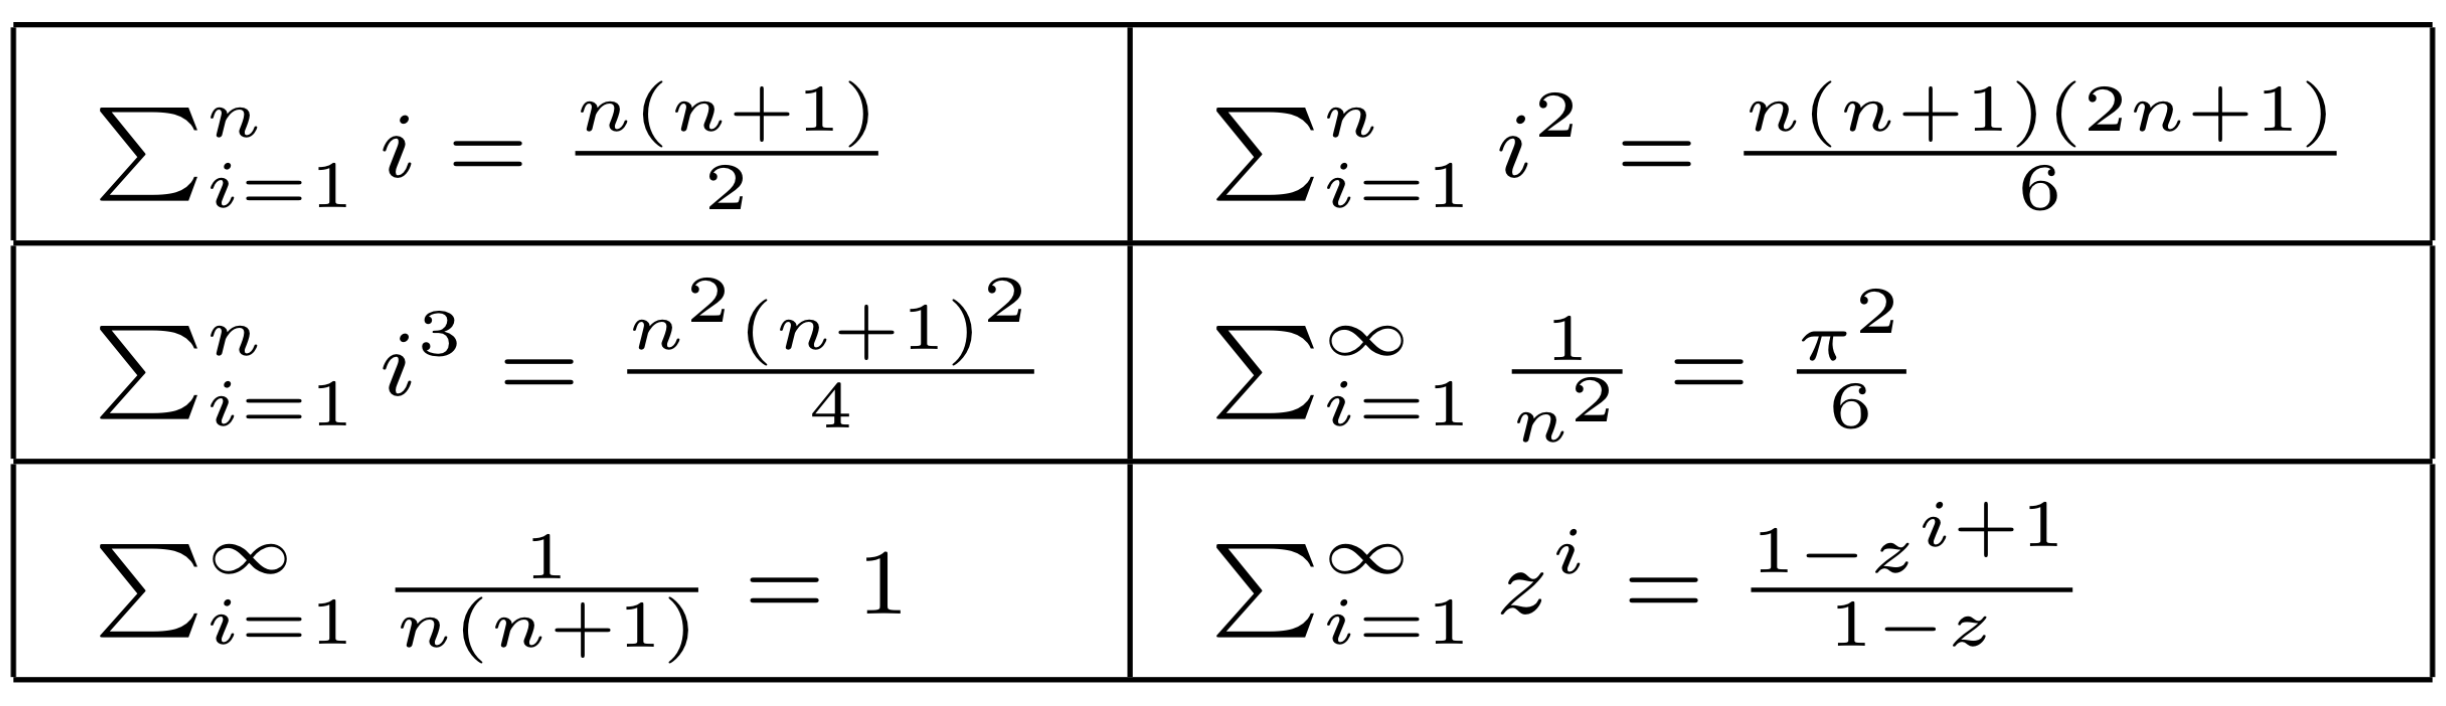
\includegraphics[width=0.4\linewidth]{./assets/series.png}
\begin{multicols}{2}
    \shade{ForestGreen}{\tr{Common limits}{Häufige Grenzwerte}}

    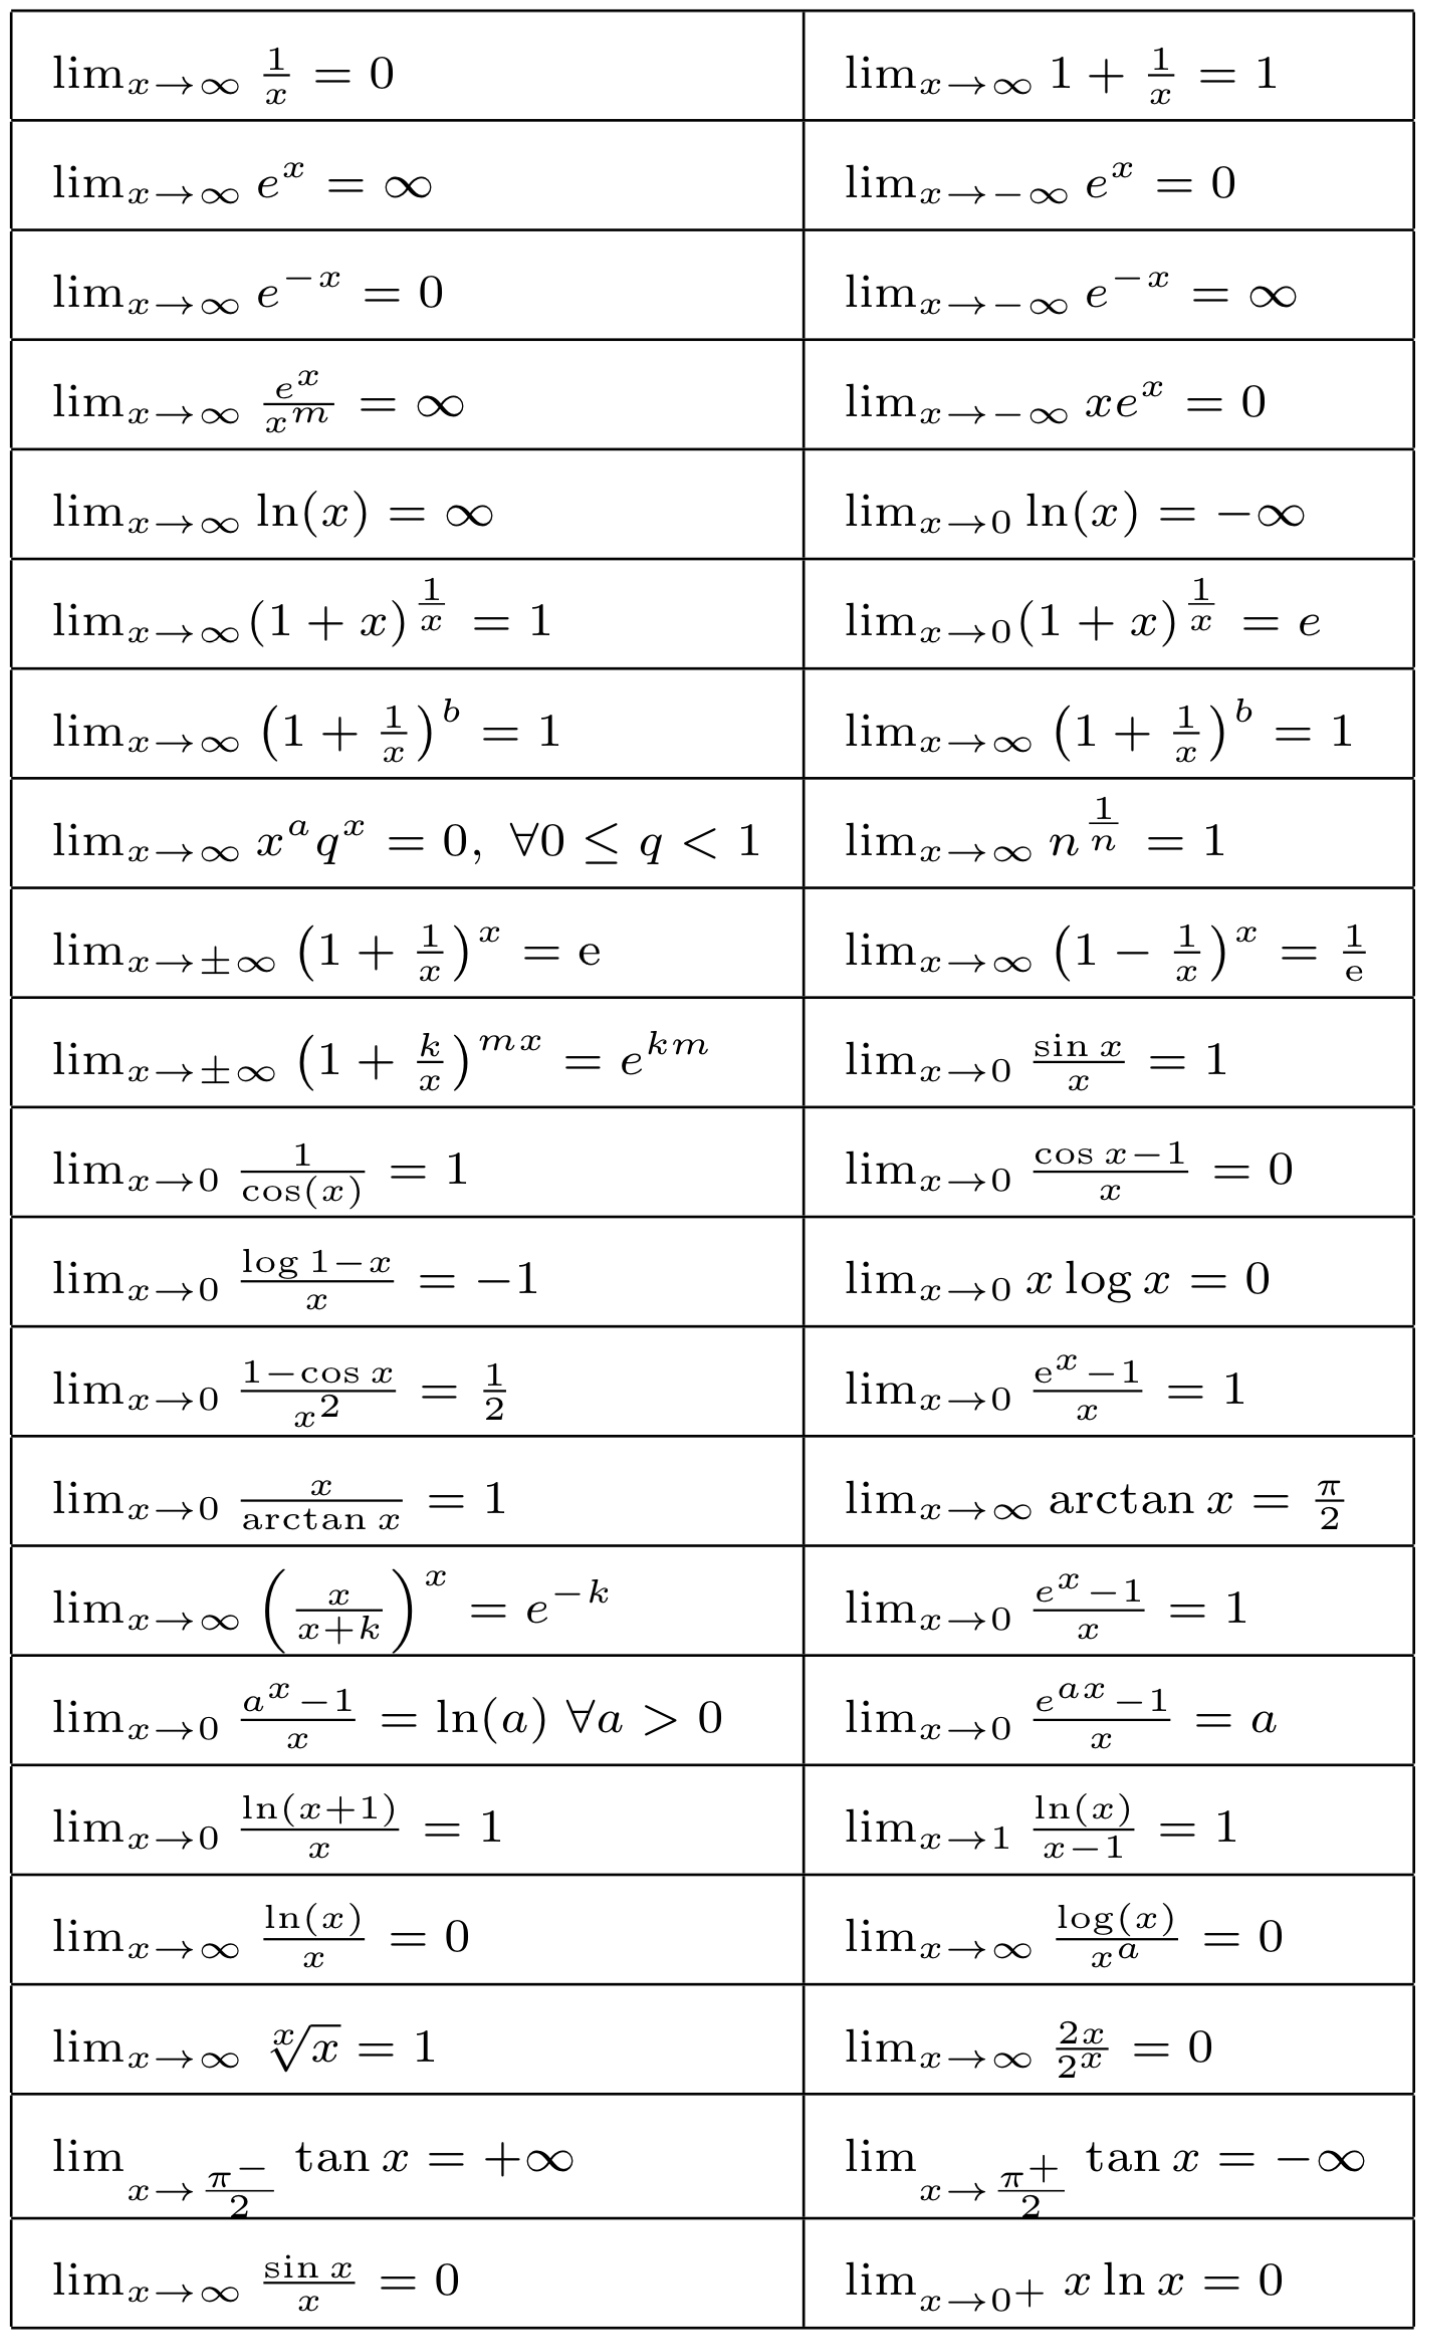
\includegraphics[height=0.5\textheight]{./assets/limits.png}


    \shade{ForestGreen}{\tr{Common Taylor Polynomials}{Bekannte Taylorreihen}}

    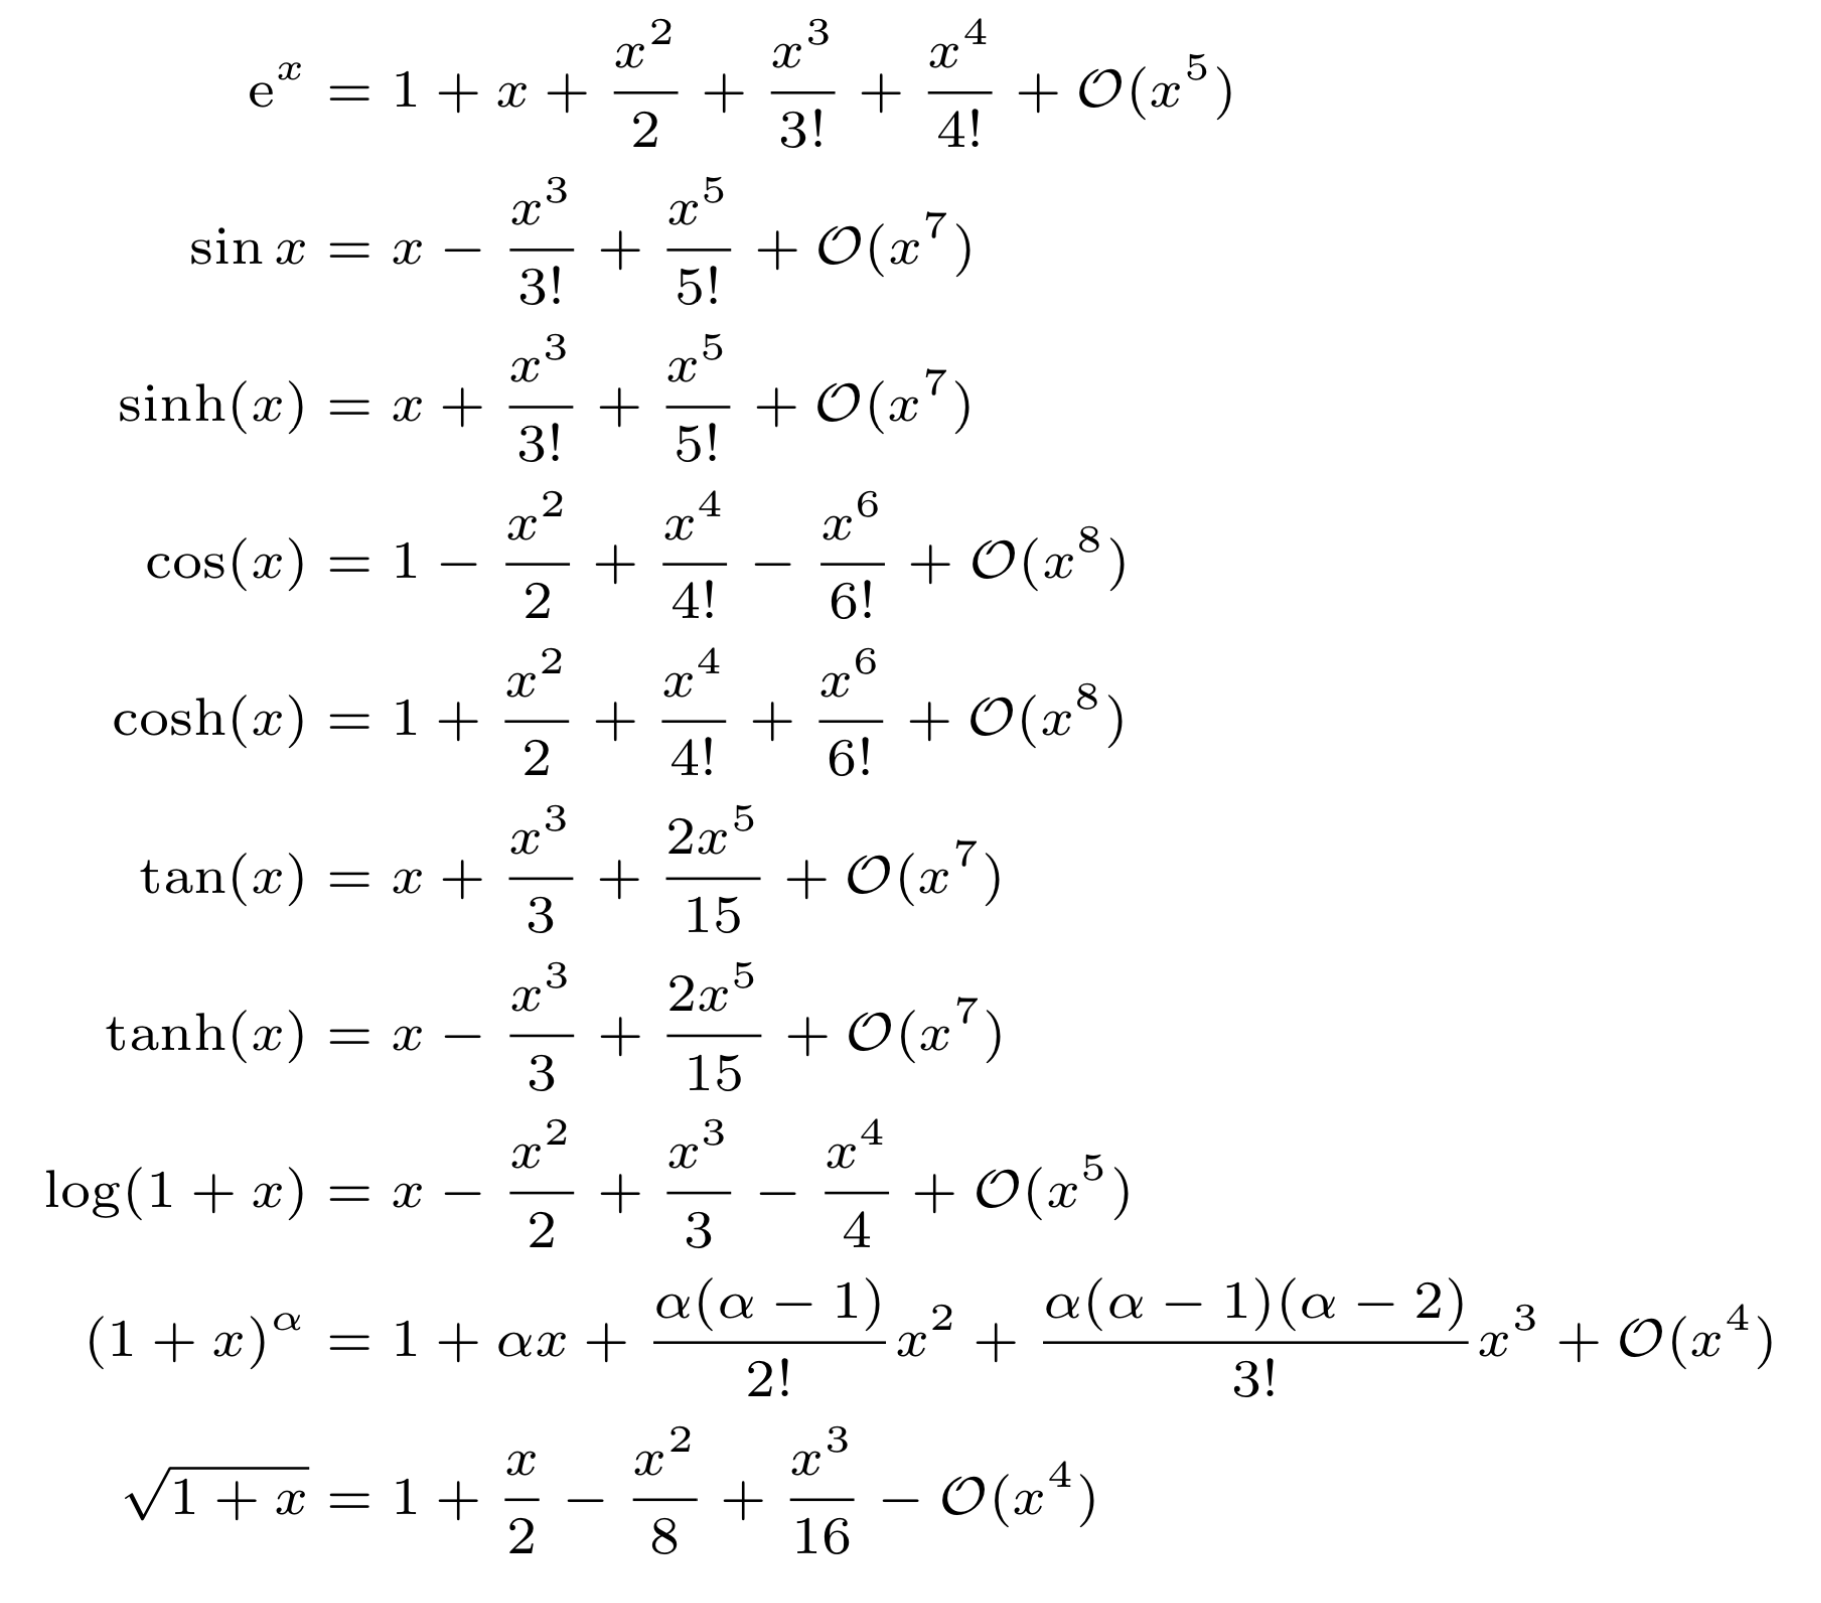
\includegraphics[width=0.8\linewidth]{./assets/taylor-polynomials.png}
\end{multicols}
